\section{Perceptron} 

  The perceptron uses a linear regression function as a plugin-classifier, inspired by the artificial modeling of a human neuron \cite{1943mcculloch}. 

  \begin{definition}[Perceptron]
    The \textbf{perceptron model} is a discriminative linear classifier that assigns 
    \begin{equation}
      f_w (x) = \begin{cases} 1 & \text{ if } w^T x + b \geq 0 \\ -1 & \text { if } w^T x + b < 0 \end{cases}
    \end{equation}
    where we have chosen to label class $C_1 = 1$ and $C_2 = -1$. 
  \end{definition}

  Note that unlike linear regression (and logistic regression, as we will see later), the perceptron is not a probabilistic model. It is a \textit{discriminant function}, which just gives point estimates of the classes, not their respective probabilities. Like logistic regression, however, it is a linear model, meaning that the decision boundary it creates is always a linear (affine) hyperplane. 

  To construct the surrogate loss function, we would want a loss that penalizes not only if there is a misclassification, but how \textit{far} that misclassified point is from the boundary. Therefore, if $y$ and $\hat{y} = f_w (x)$ have the same sign, i.e. if $y f_w (x) > 0$, then the penalty should be $0$, and if it is $< 0$, then the penalty should be proportional to the orthogonal distance of the misclassified point to the boundary, which is represented by $-wT x y$ (where the negative sign makes this cost term positive). 

  \begin{definition}[Surrogate Loss for Perceptron]
    Therefore, our cost functions would take all the points and penalize all the terms by $0$ if they are correctly classified and by $-\mathbf{w}^T \boldsymbol{\phi}^{(n)} y^{(n)}$ if incorrectly classified. 
    \begin{equation}
      L(y, \hat{y}) = \sum_{n=1} [ -\mathbf{w}^T \boldsymbol{\phi}^{(n)} y^{(n)} ]_+ \text{ where } [f(\mathbf{x})]_+ \coloneqq \begin{cases} f(\mathbf{x}) & \text{ if } f(\mathbf{x}) > 0 \\ 0 & \text{ else } \end{cases}
    \end{equation}
    Note that this is a piecewise linear function and convex. 
  \end{definition}

  \begin{code}[Perceptron in scikit-learn]
    Let's implement this in scikit-learn, using two pipelines with different data standardization techniques to see the differences in the perceptron boundary. 

    \begin{figure}[H]
      \centering 
      \begin{lstlisting}
        from sklearn.pipeline import Pipeline 
        from sklearn.linear_model import Perceptron
        from sklearn.preprocessing import QuantileTransformer, StandardScaler

        pipe1 = Pipeline([ 
            ("scale", StandardScaler()), 
            ("model", Perceptron())
        ])

        pipe2 = Pipeline([
            ("scale", QuantileTransformer(n_quantiles=100)), 
            ("model", Perceptron())
        ])
      \end{lstlisting}
      \caption{} 
    \end{figure}

    \begin{figure}[H]
      \centering
      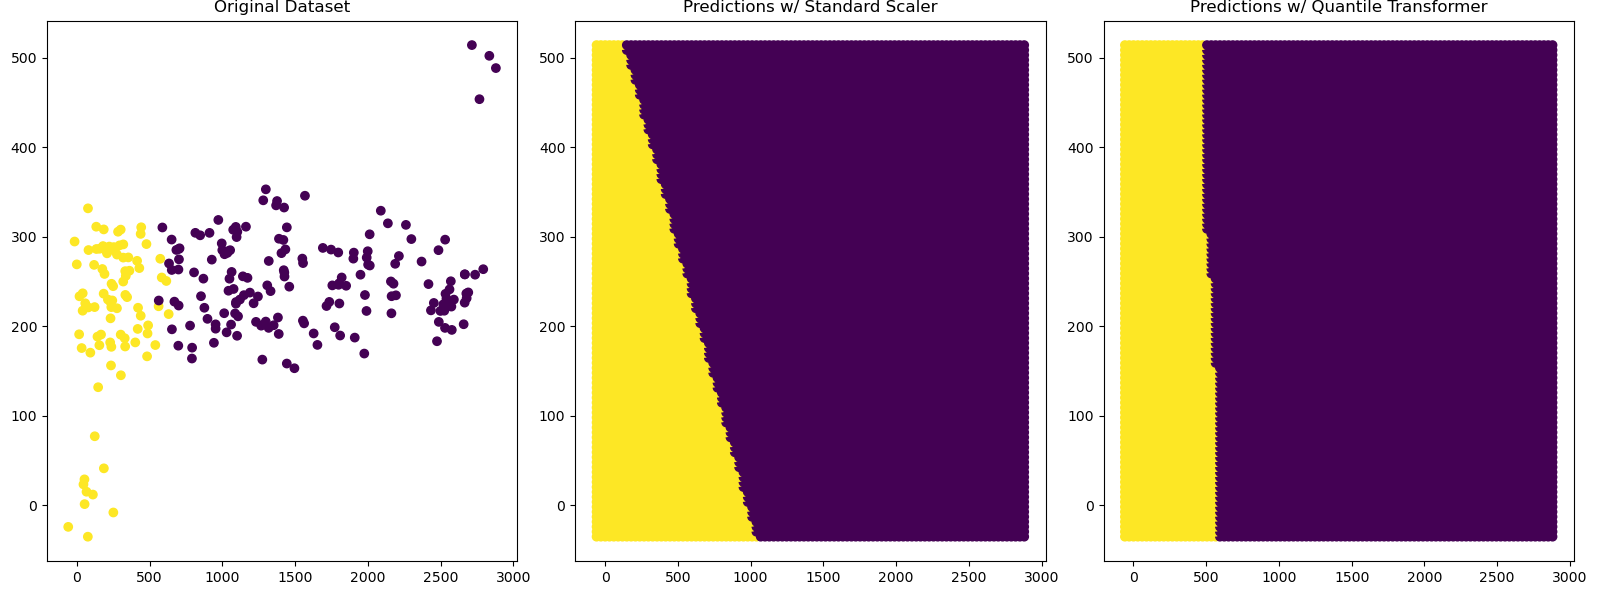
\includegraphics[scale=0.35]{img/Perceptron.png}
      \caption{Perceptron Trained on Different Standardized Data}
    \end{figure}
  \end{code}

